\chapter{实验误差}
\section{误差与全微分}
我们做实验的时候一般是直接测量一些物理量,用它们算出另一些物理量。比如测得的物理量是$x,y$,算出的物理量$f$可以表示为$f(x,y)$。如果$x$的测量值与真实值相差$\Delta x$,而$y$是准确的,那么$f$与真实值相差$\Delta f=\frac{\partial f}{\partial x} \Delta x$。(这里仍然不管差分算符$\Delta$、微分算符$\opd$和偏微分算符$\partial$的区别)

如果$y$的测量值与真实值相差$\Delta y$,而$x$是准确的,那么$\Delta f=\frac{\partial f}{\partial y} \Delta y$。同时考虑$\Delta x$和$\Delta y$,那么$\Delta f$就是上面两种情况之和:$\Delta f=\frac{\partial f}{\partial x} \Delta x+\frac{\partial f}{\partial y} \Delta y$。

这其实就是对$f$求全微分:$\opd f=\frac{\partial f}{\partial x} \opd x+\frac{\partial f}{\partial y} \opd y$。

上面说的是知道$x$的测量值与真实值的差,计算$f$与真实值的差。但是$x$与真实值的差实际上是不知道的,$\Delta x$一般指的是最大误差。(它是一个大于$0$的量,专业一点叫作\emph{极限不确定度})

误差可以分为系统误差和偶然误差,系统误差永远向一边偏,偶然误差可以向两边偏。这里我们主要讨论偶然误差。

考虑最坏情况,$f$的误差$\Delta f=|\frac{\partial f}{\partial x}| \Delta x+|\frac{\partial f}{\partial y}| \Delta y$。其中$\frac{\partial f}{\partial x}$和$\frac{\partial f}{\partial y}$取绝对值,也就是说这两个量即使在公式里相互抵消,计算误差时也不能抵消。

举个栗子,如图\ref{fig-length-diff},我们用刻度尺测量一个长度$l$,两头的读数分别是$x_1$和$x_2$,那么$l=x_2-x_1$,但是$\Delta l=\Delta x_2+\Delta x_1$。
\begin{figure}[htb]
\centering
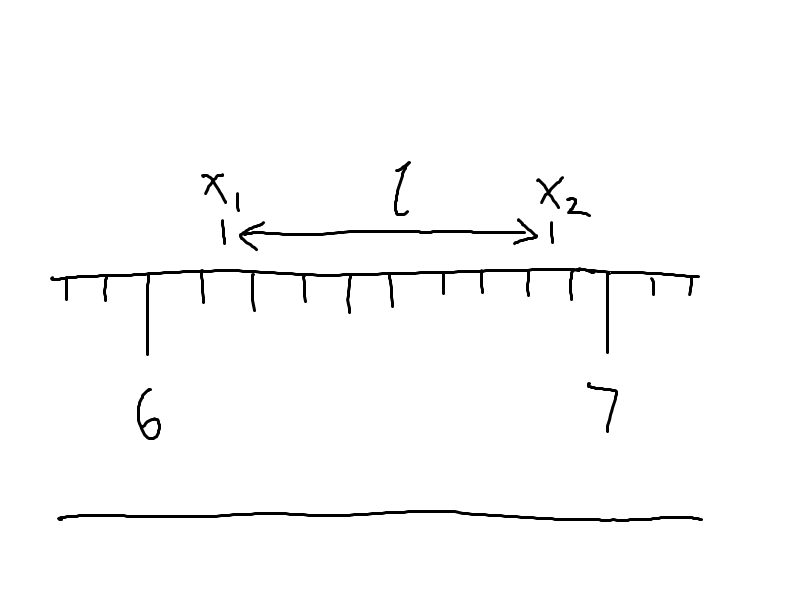
\includegraphics[scale=0.5]{fig/length-diff.png}
\caption{一把肥硕的尺子}
\label{fig-length-diff}
\end{figure}

再比如伏安法测电阻,$R=\frac{U}{I}$,$\Delta R=\frac{1}{I} \Delta U+\frac{U}{I^2} \Delta I$。

注意:用这种方法计算$f(x,y)$的误差,要求$x$与$y$无关。我们的物理课上发生过这么一件事:用打点计时器测加速度,有人用前半段纸带算一个加速度$a_1$,后半段纸带算一个加速度$a_2$,然后把$a_1$和$a_2$平均,结果发现误差比想象的大。事实上计算$a_1$和$a_2$用的一些点是相同的,$a_1$和$a_2$就是相关的,不能直接计算平均后的误差。

两个物理量是否相关有时候并不显然,需要通过实验来检验:测量多组$x$和$y$,看看它们之间有没有什么统计规律。(很多生物实验干的就是这样的事情)
\section{绝对误差与相对误差}
上面说的误差都是绝对误差,有时还会用到相对误差,比如$x$的相对误差为$|\frac{\Delta x}{x}|$。(严格来说分母应该是真实值,我们一般用测量值代替)

我们说的误差有时指绝对误差,有时指相对误差,要看具体情况。几个量加减的时候计算绝对误差比较方便,几个量乘除的时候计算相对误差比较方便。比如把上面伏安法测电阻的式子除以$R$得到$\frac{\Delta R}{R}=\frac{\Delta U}{U}+\frac{\Delta I}{I}$。

如果$x$是直接测量的量,那么在$\Delta x$固定的情况下,$x$越大,相对误差越小,所以我们一般要求被测量大于量程的$\frac{1}{3}$。

但是如果$x$是算出来的量,减小相对误差的方法就没有这么显然了。比如上面用刻度尺测长度,如果想减少$x_1$和$x_2$的相对误差,可以把东西放在离零刻度线很远的地方量,这样$x_1$和$x_2$都很大。但是这样做并没有什么用,因为$l$和$\Delta l$都不变,$l$的相对误差也不变。
\section{传感器的灵敏度}
现在来看一道题:如图\ref{fig-temp-detector},$R_T$是一个热敏电阻,温度为$T$时阻值为$R_T(T)$,$\frac{\partial R_T}{\partial T}>0$,也就是说温度越高阻值越大。$R_0$是定值电阻。$V$是理想电压表,内阻无穷大。$E$是理想电源,内阻忽略(有内阻也可以合到$R_0$里)。
\begin{figure}[htb]
\centering
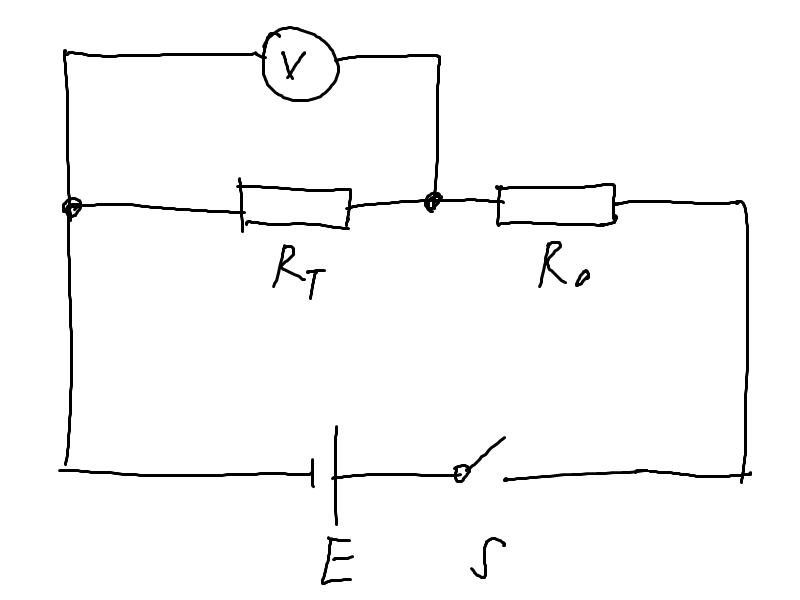
\includegraphics[scale=0.5]{fig/temp-detector.png}
\caption{一个肥硕的电路}
\label{fig-temp-detector}
\end{figure}

这个电路可以作为温度传感器,$V$的示数为$U_T(T)=\frac{E R_T}{R_T+R_0}$,温度越高,$U_T$越大。

温度改变$\Delta T$时,$\Delta U_T=\frac{E R_0}{(R_T+R_0)^2} \frac{\partial R_T}{\partial T} \Delta T$。我们把$\frac{\Delta U_T}{\Delta T}=\frac{E R_0}{(R_T+R_0)^2} \frac{\partial R_T}{\partial T}$称为传感器的灵敏度,$\Delta T$相同时,灵敏度越大,$\Delta U_T$就越大。

$\frac{\partial R_T}{\partial T}$越大,灵敏度就越大,这符合直觉。还可以发现常温下的电阻$R_T$越大,灵敏度越小。如果可以选择不同的$R_0$,那么$R_0=R_T$时灵敏度最大,因为
\begin{equation*}
\frac{R_0}{(R_T+R_0)^2}=\frac{1}{R_0+\frac{R_T}{R_0}+2 R_T}
\end{equation*}
\section{有效数字}
上面说了通过被测量的最大误差计算结果的最大误差的方法。有效数字是一种更加方便但不精确的方法,相当于把绝对误差当成最后一位数字。比如$x=1.23 \times 10^3$其实表示$1.225 \times 10^3 \le x <1.235 \times 10^3$,绝对误差为$0.01 \times 10^3=10$。有效数字从最左边的不为$0$的数字到最右边的数字为止,这些数字的个数称为有效位数。

几个量加减的时候有效数字取绝对误差大的,几个量乘除的时候有效数字取相对误差大的(也就是有效位数少的)。比如$1.23 \times 10^3+8.9 \times 10^1=1.32 \times 10^3$,而$1.23 \times 10^3 \times 8.9 \times 10^1=1.1 \times 10^5$。

一般认为幂函数、指数函数、对数函数和三角函数的有效位数就是自变量的有效位数。如果需要更精确,还是老老实实算导数吧。

如果用同一个仪器测量多组数据,它们的有效位数不同(比如测电流从$1.2 \unit{A}$测到$12.3 \unit{A}$),有时候会统一按照有效位数最多的值计算(传说是为了让结果更好看),更精确的实验会单独计算每组数据的误差。

画图时坐标轴的有效位数有人认为要与测得的数据相同,有人认为应该根据方格纸的最小刻度和估读确定,更精确的实验会在每个数据点附近标出它的误差范围。
\section{误差的来源}
$x$是测量得到的值,那么怎么确定最大误差$\Delta x$呢?偶然误差可以分为两部分:一是统计误差,也就是多次测量时每次测得的值不同造成的;二是仪器误差,也就是每次测量时仪器的最小刻度等等造成的。(专业一点叫作\emph{A类不确定度}和\emph{B类不确定度})

仪器误差比较容易理解,一般取的是仪器的最小刻度,要估读就取估读出的最小刻度。但是也有一些约定俗成的取法,比如钢尺是$0.1 \unit{mm}$,游标卡尺是$0.02 \unit{mm}$,螺旋测微器是$0.004 \unit{mm}$,秒表是$0.5 \unit{s}$(人的反应时间)。专业的仪器生产厂商会在仪器上标出仪器误差。

讲统计误差需要一些统计学的知识。比如你用刻度尺测一只虫子的长度,测量$3$次分别是$1.05 \unit{cm}$,$1.04 \unit{cm}$,$1.06 \unit{cm}$,你觉得不够,再测量$3$次分别是$1.02 \unit{cm}$,$1.08 \unit{cm}$,$1.05 \unit{cm}$。前$3$次和总共$6$次的平均值都是$1.05 \unit{cm}$,而且前$3$次的结果相互之间比较接近,统计误差应该比较小。

这里我不打算讲统计误差的计算公式,可以粗略地认为是这些数据的标准差。(也就是方差开根号,但是严格的定义有所不同)

但是!我们认为测$6$次比测$3$次更好。虽然统计误差变大了,但是真实值更有可能落在误差范围内。如果只测$3$次,你得到的测量值可能如图\ref{fig-error-range},$3$次的测量值都比真实值大。而且相互接近,完全有可能出现这样的偶然情况。(在没有系统误差的前提下)如果增加测量次数,可能会测出偏小的值,这样真实值就更有可能落在误差范围内。
\begin{figure}[htb]
\centering
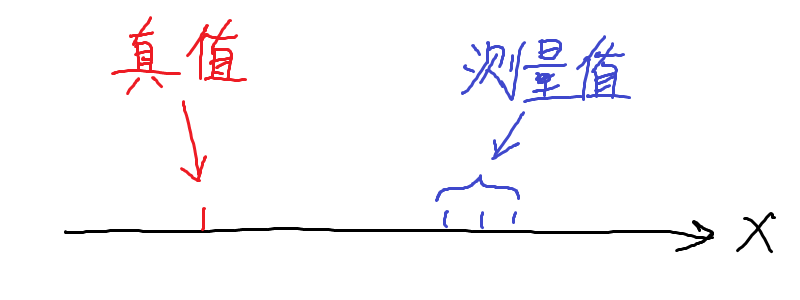
\includegraphics[scale=0.5]{fig/error-range.png}
\caption{一个RP不足的同学测出的结果}
\label{fig-error-range}
\end{figure}

多次测量取平均值并不能减小仪器误差。比如$\overline{x}=\frac{1}{n}(x_1+x_2+\dots+x_n)$,而每次测量的仪器误差$\Delta x_1,\Delta x_2,\dots,\Delta x_n$都是$\Delta x$,那么$\Delta \overline{x}=\frac{1}{n} n \Delta x=\Delta x$。多次测量取平均值也不一定会减小统计误差,它的真正意义是让平均值和统计误差变得更合理,接下来仔细讲一下这件事情。

(许多高考实验题的误差范围都是出题人一拍脑袋想出来的,说明他们的物理素养不高)
\section{正态分布;置信度}
如果对一个物理量进行多次测量,测量值会满足一定的分布。最常见的是正态分布,又叫高斯分布:(什么你要萝莉分布?我这里没有)
\begin{equation*}
P(x)=\frac{1}{\sqrt{2 \pi} \sigma} \rme^{-\frac{(x-x_0)^2}{2 \sigma^2}}
\end{equation*}

这个式子看起来很厉害,但是不要怕,不要怕,不要怕。它的图像大致如图\ref{fig-gaussian}:
\begin{figure}[htb]
\centering
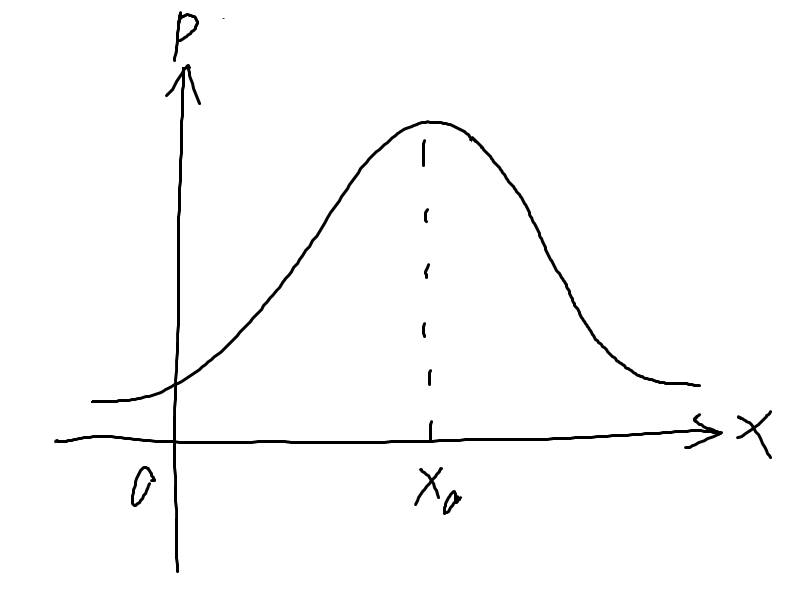
\includegraphics[scale=0.5]{fig/gaussian.png}
\caption{画得好像不是很对称}
\label{fig-gaussian}
\end{figure}

如果一个物理量的真实值为$x_0$,对它进行测量,测量值为$x$的概率就是$P(x)$。进行的测量次数越多,平均值就越接近$x_0$,标准差越接近$\sigma$,详细的证明以后再讲。(需要很复杂的积分,估计是有生之年)

$x_0$和$\sigma$这两个参量可以确定一个正态分布,$x_0$确定峰的左右位置,$\sigma$确定峰的宽度。因为概率的归一化,只要峰的宽度确定了,峰的高度就确定为$\frac{1}{\sqrt{2 \pi} \sigma}$。

$\sigma$是由被测量、仪器、测量方法等等决定的。比如一只虫子在$1 \unit{cm}$范围内抖动,你测量它的位置,$\Delta x$就大约有$1 \unit{cm}$,如果测出来$\Delta x$只有$0.01 \unit{cm}$反而不符合事实,但是我们仍然可以测出虫子位置的平均值。再比如一根圆柱体的表面凹凸不平,你在不同方向测量它的直径就会得到不同的值。所以说统计误差不是越小越好,多次测量取平均值可以让平均值和统计误差变得更合理。

事实上不同的仪器有不同的误差分布,正态分布只是一个近似。比如测量长度怎么也不可能小于$0$,但是正态分布在小于$0$的地方还是有的,只是概率很小而已。对一些标准量进行测量可以证明,正态分布在大多数情况下是很好的近似。比如扔$n$次硬币有$k$次正面朝上的概率为$P(k)$(没错就是二项式分布),当$n$很大时,$P(k)$接近正态分布,$k=\frac{n}{2}$的地方最大,向两边减少。

如果已知$x_0$和$\sigma$,可以求出$x$为某个值$x_1$的概率。但是做实验做的其实是相反的事情:已知测量值$x_1,x_2,\dots,x_n$,假设$x$满足正态分布,求$x_0$和$\sigma$分别为某个值$x_{0 1}$和$\sigma_1$的概率。通过解含有随机变量的方程可以把$x_0$和$\sigma$的分布函数算出来,但是这个计算很复杂。

知道了$x_0$和$\sigma$的分布,就可以计算置信度CI,它可以描述测量结果的准确程度。比如置信度为95\%表示区间$(\overline{x}-\Delta x,\overline{x}+\Delta x)$有95\%的可能性覆盖到了真实值$x_0$。

置信度与测量次数$n$和最大误差$\Delta x$有关,$n$越大,或者$\Delta x$越大,那么置信度越大。具体的计算也很复杂,实际工作中一般可以查表。

实验永远不能100\%保证真实值是多少,只能给出这样的一个概率,除非$\Delta x$无穷大,覆盖整条数轴。现代粒子物理的置信度一般是90\%或者95\%,火箭之类的精密工程甚至可以达到99.9999\%。
\section{仪器的分辨率}
仪器的分辨率大致就是最小刻度,也有些地方的定义是最小刻度的倒数。最小刻度不可能无限减小,总有一些物理规律限制它。(所以分辨率应该是越小越好还是越大越好呢)

光学实验中限制分辨率的一个重要原因是衍射。比如显微镜需要用光照亮物体(或者电子束衍射之类的),如果用可见光,波长约为$500 \unit{nm}$,比波长更小的物体衍射现象就会很明显,看不清楚。如果减小波长,光的衍射现象会减弱,但是光的动量就变大了,撞到物体上对它的影响会增强,测量结果会受到量子力学中不确定性原理$\Delta x \Delta p \le \frac{\hbar}{2}$的限制。

有些实验仪器需要用透镜把光汇聚到一个点上,但是因为衍射,这个点不可能无限小。道理跟小孔成像是一样的,虽然透镜比小孔大得多,但是衍射现象仍然存在。如果光的波长是$\lambda$,透镜的大小是$D$,焦距是$f$,那么衍射范围的大小$d=\frac{\lambda f}{D}$。

这里透镜的大小(专业一点叫\emph{线度})可以是圆形的直径、半径,或者正方形的边长等等,只要量纲是长度就行,先不管前面的系数。可以看出,$\lambda$越大,$D$越小,衍射就越明显。

在精密的力学实验中,限制分辨率的一个重要原因是热运动。比如用一把尺子测一根杆子的长度,要把整个实验装置放到低温环境中,来减小尺子和杆子的热运动。但是!你还记得前面讲的热波长吗?温度降低,尺子和杆子的热波长就会增大,测量结果仍然受到不确定性原理的限制。

前面说的都是空间分辨率,计时的仪器也有时间分辨率。比如高考范围内的打点计时器每隔$0.02 \unit{s}$打一个点,如果每两个点的距离相等,我们就认为物体在匀速运动。其实如果物体的速度在快速变化,而变化的时间小于$0.02 \unit{s}$,用打点计时器是看不出来的。(如果你熟悉傅立叶变换,可以认为打点计时器过滤了速度的高频分量)

多次测量取平均值可以理解为牺牲时间分辨率来换取空间分辨率。
